\section{Price analysis}\label{Sec:Price analysis}

One of the core factors in the choice of the property to book is its price, being one of main drivers of customers' behaviors \citep{liang2018understanding}. Therefore one may want to try and see what properties' attributes influence its value.

We start in subsection \ref{subsec:corr} by calculating the correlation of all the other variables with respect to price. Then we try in subsection \ref{subsec:lm} to run a linear regression on price to look what variables are statistically relevant and how much they affect the price.


\subsection{Correlation with price}\label{subsec:corr}

Since we are only interested in the correlation with price, a classic correlation plot like the one in figure \ref{figure:corrplot} may not be the most easily readable in this case, especially because of the large number of variables.

-- UNDERSTAND HOW TO PUT IMAGE embedded in text

\begin{figure}[H]
\begin{center}
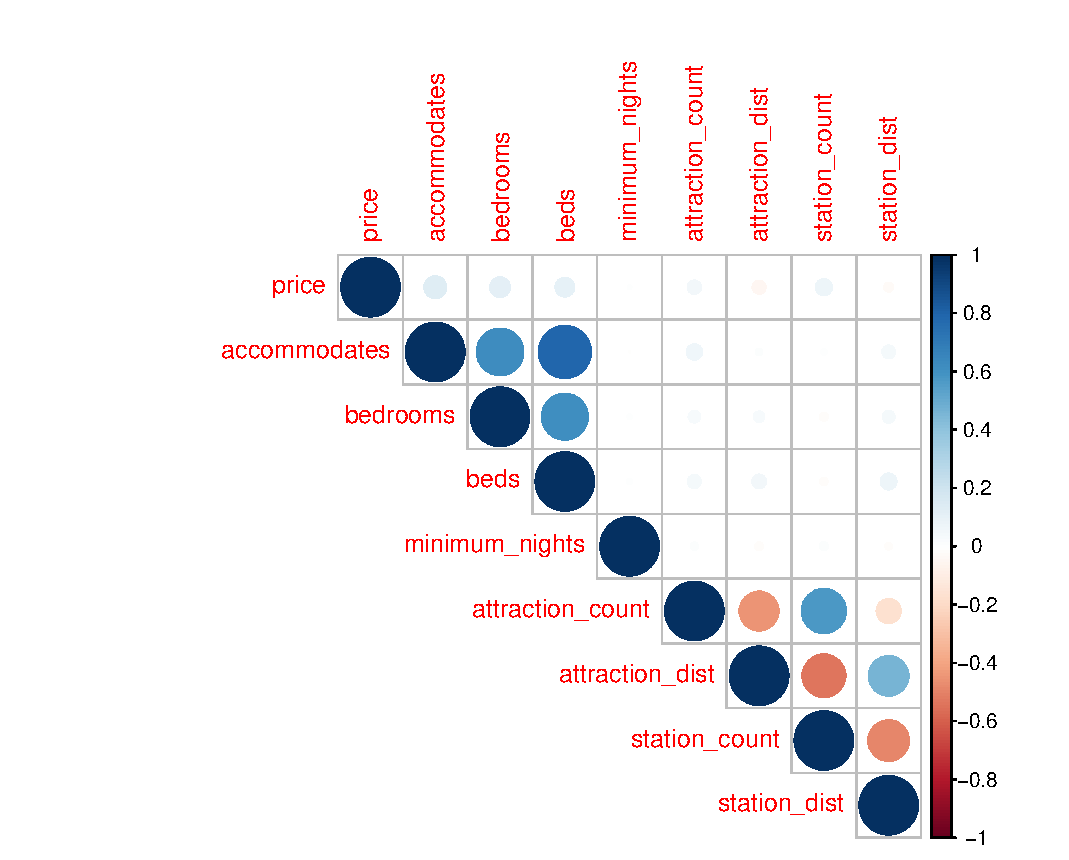
\includegraphics[width=0.5\textwidth]{corrplot.pdf}
\caption{Correlation plot with the function  \texttt{corrplot} from the package \texttt{corrplot} }
\label{figure:corrplot}
\end{center}
\end{figure}

In fact, categorical variables first need to be transformed into many dummy variables in order to calculate the correlation. The function \texttt{from\_row\_to\_col} will be used to achieve this result. It creates dummy variables for all factor levels by creating a column of 1s, spreading it across so many columns as factor levels and filling the empty rows in the columns with 0s.


\lstinputlisting[language=R, firstline=2, escapechar=|, caption={|\textbf{\href{https://github.com/silvia-ventoruzzo/SPL-WISE-2018/blob/master/Helpers/from_row_to_col.R}{from\_row\_to\_col.R}}|}]{../Helpers/from_row_to_col.R}


\begin{figure}[H]
\begin{center}
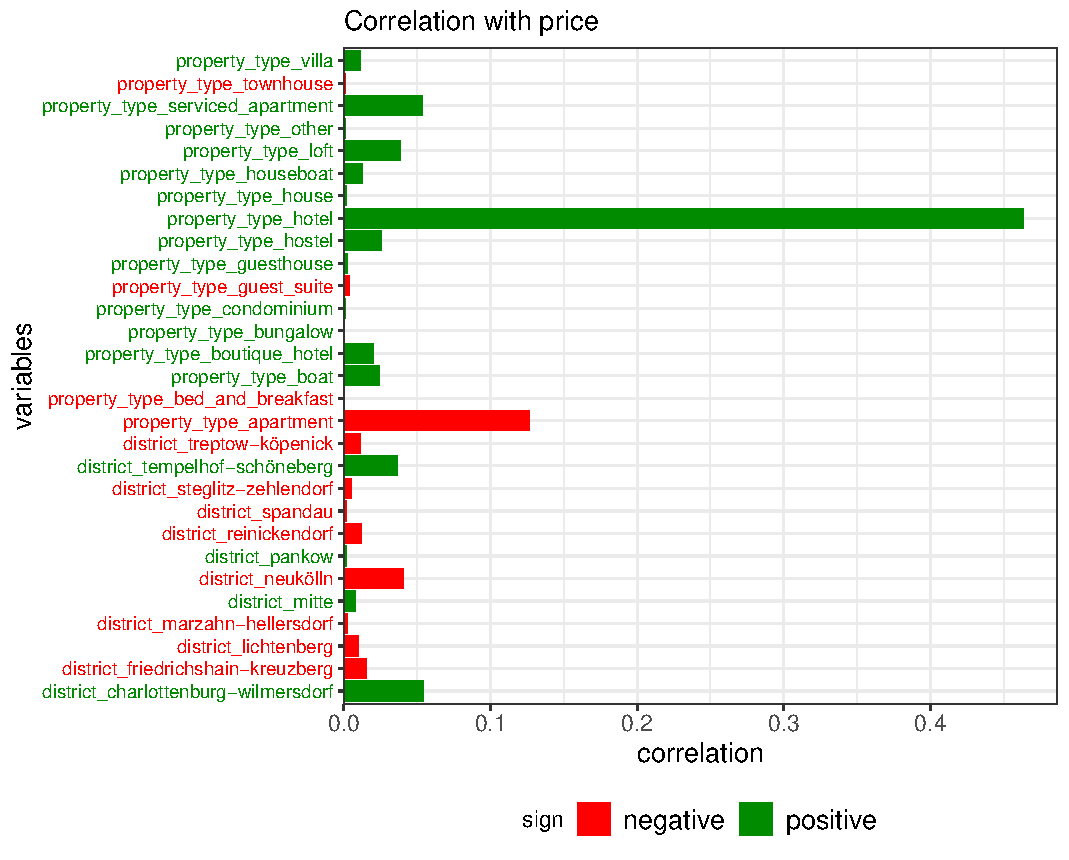
\includegraphics[width=0.8\textwidth, keepaspectratio]{price_correlation.pdf} \\
\caption{Sample of plot of correlation with price}
\label{figure:pricecorr}
\end{center}
\end{figure}



\subsection{Linear regression on price}\label{subsec:lm}

As pointed out in \cite{wang2017price} linear regression is used to describe possible linear relationships between a dependent variable and one or multiple independent variables.

In this case we will look for the relationship that the properties' attributes have on their price. 

